\documentclass[a4paper]{article}

\usepackage[portuguese]{babel}
\usepackage{comment}
\usepackage[T1]{fontenc}
\usepackage[utf8]{inputenc}
\usepackage{hyperref}
\usepackage{graphicx}
\usepackage{float}
\usepackage{multirow}
\usepackage{indentfirst}
\usepackage[hypcap]{caption} % makes \ref point to top of figures and tables

\begin{document}

\begin{titlepage}

	\begin{center}

		
\includegraphics[width=6cm]{./title}\\[3cm]

		\textsc{\LARGE Redes Móveis e Sem Fios}\\[1.5cm]

		\textsc{\Large Relatório intermédio  }\\[1.5cm]
		
		
		\textsc{Development of Internet of Things sensor monitoring based on SigFox, Arduino and Android }\\[1.5cm]
		



		


		\noindent
		\begin{minipage}{0.4\textwidth}
			\begin{flushleft} \large
				Bernardo Gomes, 75573
			\end{flushleft}
		\end{minipage}
		\begin{minipage}{0.4\textwidth}
			\begin{flushright} \large
				Diogo Martins, 75462
			\end{flushright}
		\end{minipage}

		\vfill

		{\large \today}


	\end{center}

\end{titlepage}
\hypersetup{%
    pdfborder = {0 0 0}
}

\tableofcontents
\pagenumbering{gobble}
\pagebreak

\pagenumbering{arabic}
\section{Objectivo}

O objectivo do projecto é o desenvolvimento de um sistema de monitorização de temperatura. 

O sistema, deverá ser baseado num sensor de temperatura associado a um dispositivo \textit{Arduino (Akeru 3.3)}, que irá comunicar as suas medições a um servidor \textit{SigFox}, armazenando-as na \textit{Cloud}.

Na óptica do utilizador, irá ser desenvolvida uma aplicação em ambiente \textit{Android}, que fornecerá os dados presentes na \textit{Cloud} com uma apresentação \textit{user friendly}. Pretende-se ainda que seja possível que o utilizador registe um novo dispositivo a monitorizar na aplicação, bem como definir alarmes para certos valores de temperatura.


\section{Solução encontrada}

Tal como referido na secção anterior, a monitorização da temperatura e da qualidade de medição do sensor, irá ser feita pelo utilizador com recurso à aplicação, mas tendo a \textit{Cloud SigFox} como intermediária.

Por forma a que os dados de cada utilizador sejam independentes do dispositivo utilizado, foi construída uma base de dados adicional, que guarda informação de \textit{login} bem como dos \textit{devices} e os \textit{thresholds} de alarme de cada utilizador.

A arquitectura será então a apresentada na figura \ref{fig:general}:
\vspace{2mm}

\begin{figure}[hb]
  \centering
  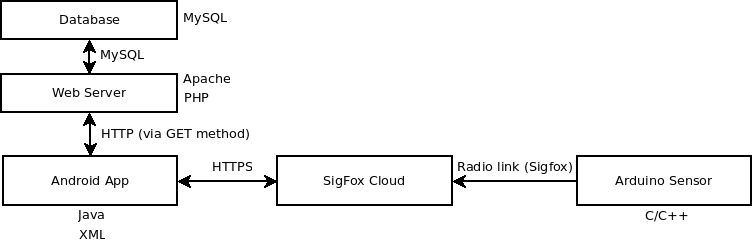
\includegraphics[scale=0.45]{general.png}
  \caption{Arquitectura geral}
  \label{fig:general}
\end{figure}

\subsection{Aplicação \textit{Android}}

A aplicação \textit{Android}, com a qual o utilizador irá ter contacto directo, será constituída por cinco actividades:

\begin{itemize}
\item \textit{MainActivity};
\item \textit{CreateLogActivity};
\item \textit{LogsActivity};
\item \textit{NewAlarmActivity};
\item \textit{AddDeviceActivity}.
\end{itemize}

As relações entre as actividades descritas, encontram-se representadas na figura \ref{fig:app_android_geral}.

\vspace{5mm}

\begin{figure}[hb]
  \centering
  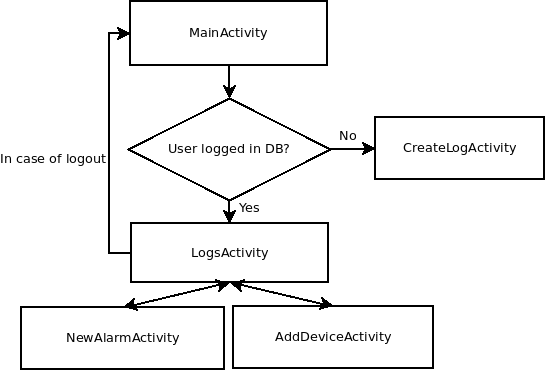
\includegraphics[scale=0.40]{App_geral.png}
  \caption{Arquitectura da aplicação \textit{Android}}
  \label{fig:app_android_geral}
\end{figure}

A \textit{MainActivity} tem como objectivo perguntar ao utilizador o nome com o qual está registado na rede, realizando \textit{queries} à base de dados com as informações do utilzador. No caso de existir registo prévio, as informações são armazenadas num ficheiro que irá funcionar como \textit{cache} na aplicação e é lançada a \textit{LogsActivity}. Caso o utilizador na tenha registo, é lançada a \textit{CreateLogActivity} para registar o novo utilizador. 

A actividade de registo de um utilizador (\textit{CreateLogActivity}), terá apenas três campos de inserção de texto: \textit{username, password} e \textit{devicetype-id}. Estes parâmetros são gravados no ficheiro de texto descrito anteriormente, bem como na base de dados central. De seguida, a aplicação irá lançar a \textit{LogsActivity}.

A actividade de visualização da informação da \textit{Cloud} (\textit{Logs}), é constituída por duas \textit{threads} principais. A primeira consiste na obtenção das mensagens do dispositivo por pedidos HTTPS (GET) periódicos, de acordo com a informação de registo do utilizador e que é actividada por uma \textit{checkbox}. Posteriormente a resposta será enviada para a \textit{thread} principal (da API) que a disponibiliza ao utilizador. No caso de a \textit{checkbox} não estar activa, os pedidos podem ser efectuados apenas ao clicar no botão de pedido de informação. O esquema desta actividade está descrito na figura \autoref{fig:app_logs}.

Esta actividade tem ainda a opção de registar um novo dispositivo para monitorização, bem como adicionar um novo alarme de temperatura. No caso de um \textit{threshold} de temperatura, lido da base de dados no início da aplicação, ser ultrapassado, a \textit{thread} que realiza o \textit{parsing} da informação deverá lançar uma notificação ao utilizador.

À semelhança da actividade \textit{CreateLogActivity}, as actividades \textit{AddDeviceActivity} e \textit{NewAlarmActivity} serão apenas compostas por campos de texto. Após o registo num ficheiro e na base de dados das informações recolhidas, estas actividades irão retornar no \textit{stack}, voltando à actividade anterior.

No caso de o utilizador pretender fazer \textit{logout}, é lançada a \textit{MainActivity}, por forma a que seja possível iniciar a sessão com outro \textit{username}.

\begin{figure}[H]
  \centering
  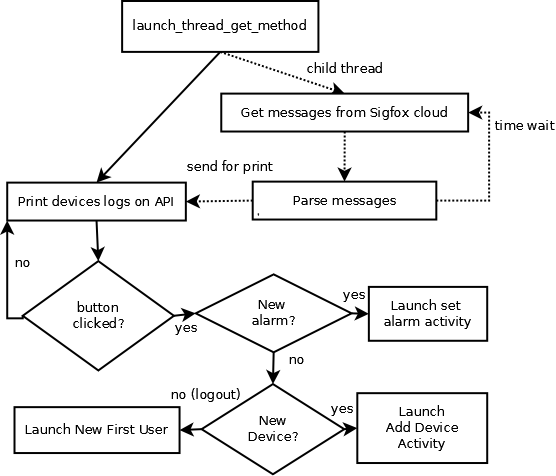
\includegraphics[scale=0.40]{ShowLogs.png}
  \caption{Arquitectura da actividade \textit{Logs}}
  \label{fig:app_logs}
\end{figure}

\subsection{Servidor \textit{SigFox}}

O papel deste servidor é o armazenamento da informação medida pelo sensor e a recepção de pedidos por parte da aplicação \textit{Android}. Consoante o tipo de pedido, irá realizar uma resposta em \textit{JSON} com as informações das medições.

Em termos de implementação para o projecto, foi apenas necessário conhecer a forma como os pedidos devem ser realizados bem como o formato de resposta.

\subsection{Sensor Arduino}

O sensor deverá realizar medições periodicamente enviando-as para a \textit{Cloud SigFox}, via rádio. Sendo possível enviar 120 mensagens para a \textit{Cloud SigFox} por dia, envia-se 5 mensagens por hora logo 1 mensagem a cada 12 minutos.

\subsection{Web Server}

Por forma a realizar pedidos à base de dados, quer de leitura quer de escrita, é utilizado um \textit{Web Server} que recolhe a informação do utilizador recebida pela aplicação através do método \textit{GET} e realiza as operações respectivas na base de dados. No caso de ser realizado um pedido de informação, esta é colocado num \textit{array} que é retornado à aplicação em \textit{JSON}.

\section{Detalhes técnicos}

Para a implementação da solução descrita anteriormente, para os diferentes módulos recorreu-se às seguintes tecnologias:

Para a aplicação \textit{Android}:
\begin{itemize}
\item \textbf{MainAcitivity, CreateLogActivity, NewAlarmActivity e AddDeviceActivity} - Nestes módulos, realizam-se pedidos a um \textit{Web Server} relativamente aos dados de um dado utilizador. Assim, na \textit{MainActivity}, com base nos dados recolhidos da base de dados, é escrito um ficheiro, por forma a efectuar/consultar registos (utilizador, dispositivo ou alarme) noutras actividades. Nas restantes, o objectivo de contacto com o servidor \textit{web} é o de acrescentar informação à base de dados, sendo também o ficheiro interno actualizado. 

Para este efeito, utiliza-se a Classe \textit{FILE} presente em \textit{Android} para o armazenamento interno (\textit{cache}) e por cada pedido ao servidor, é necessária a abertura de \textit{threads} por forma a não bloquear a \textit{User Interface} (UI), recorrendo à classe \textit{AsyncTask};

\item \textbf{Logs} - Neste módulo, será essencial a abertura de uma \textit{thread}, na medida em que a UI principal não permite efectuar pedidos periódicos pelo facto de estes a poderem bloquear. Assim, caso o utiizador queira realizar pedidos periódicos, esta \textit{thread} será aberta (recurrendo à classe \textit{Thread}). Caso contrário, será apenas necessário utilizar novamente a classe \textit{AsyncTask} para os pedidos, que apenas serão realzados mediante a pressão de um botão na aplicação.

Para efectuar os pedidos HTTPS, utiliza-se a classe \textit{HttpURLConnection}. O formato destes pedidos seguem as normas descritas na REST API-Students fornecida pelo corpo docente.

Ao receber a resposta, a \textit{thread} é processada com \textit{parsing} de \textit{JSON} com recurso à classe \textit{JsonReader}. Após o processamento da resposta, é verificado se a temperatura recebida ultrapassa algum \textit{threshold} definido pelo utilizador. Em caso afirmativo, é gerada uma notificação escrita e sonora com recurso a um objecto \textit{Notification} e \textit{Ringtone}.
\end{itemize}

Para a implementação da base de dados para armazenar os registos de cada utilizador, foi seguido o seguinte modelo:

%E-R
\begin{figure}[H]
  \centering
  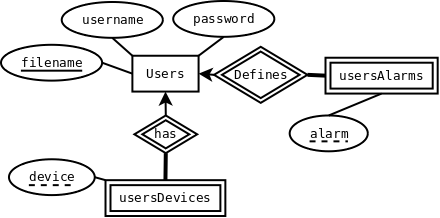
\includegraphics[scale=0.40]{DB-ER.png}
  \caption{Arquitectura da base de dados}
  \label{fig:db-er}
\end{figure}

Como tal, a base de dados irá ter três tabelas, tal como se pode verificar no \textit{script}, colocado na figura \ref{fig:db-script}, utilizado para a sua criação.

\begin{figure}[H]
  \centering
  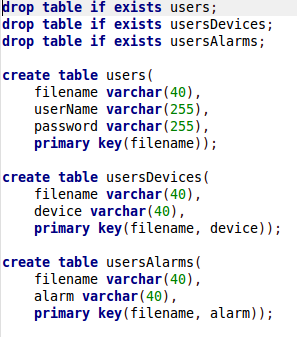
\includegraphics[scale=0.50]{DB-script.png}
  \caption{Script utilizado para a criação da base de dados}
  \label{fig:db-script}
\end{figure}

Relativamente ao alojamento da base de dados e do servidor \textit{web}, recorreu-se ao servidor do IST \textit{sigma.tecnico.ulisboa.pt}. O acesso à base de dados encontra-se protegido contra \textit{SQL Injection} utilizando-se para tal \textit{prepared statements with variable binding}, o tráfego no entanto não se encontra encriptado pois não se considerou uma ameaça de grande nível para este tipo de projecto.

Para a implementação do sensor de temperatura, recorreu-se às bibliotecas associadas ao dispositivo \textit{Akeru 3.3} disponibilizadas pelo \textit{Snootlab}. Para enviar mensagens periodicamente de 12 em 12 minutos utilizou-se a função \textit{millis()} presente em ambiente \textit{Arduino}.

\section{Verificações da solução encontrada}

Do planeamento atrás referido, foi já adiantado parte do trabalho referente à programação da aplicação, nomeadamente as actividades \textit{Welcome Screen, New First User, Set Alarm e Add Device}. De seguida são apresentadas algumas capturas de ecrã destas actividades em versão \textit{beta}.

\begin{figure}[H]
\minipage{0.32\textwidth}
  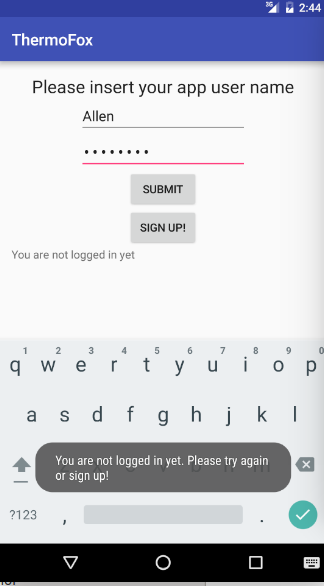
\includegraphics[width=\linewidth]{welcome.png}
  \caption{Welcome Screen}\label{fig:welcome}
\endminipage\hfill
\minipage{0.32\textwidth}
  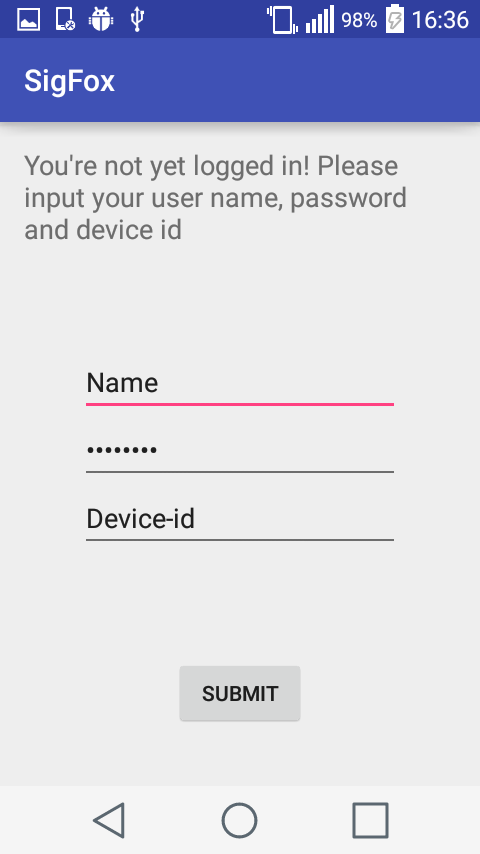
\includegraphics[width=\linewidth]{newUser.png}
  \caption{Registo de um novo utilizador}\label{fig:newUser}
\endminipage\hfill
\minipage{0.32\textwidth}%
  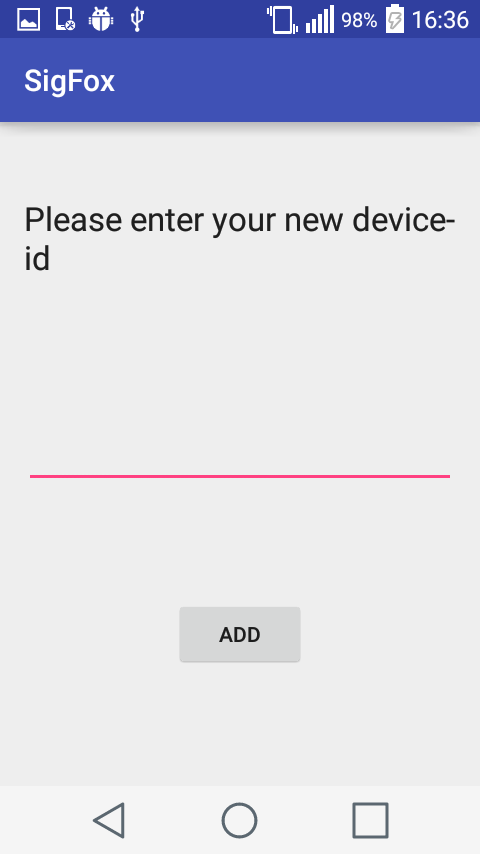
\includegraphics[width=\linewidth]{AddDevice.png}
  \caption{Registo de um novo dispositivo}\label{fig:newdev}
\endminipage
\end{figure}

\begin{figure}[H]
\minipage{0.29\textwidth}
  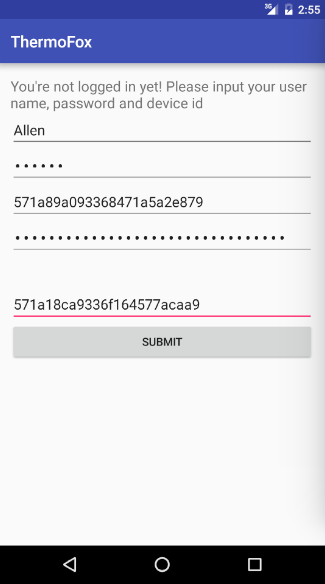
\includegraphics[width=\linewidth]{newalarm.png}
  \caption{Registo de um novo alarme}\label{fig:newalarm}
\endminipage\hfill
\minipage{0.29\textwidth}
  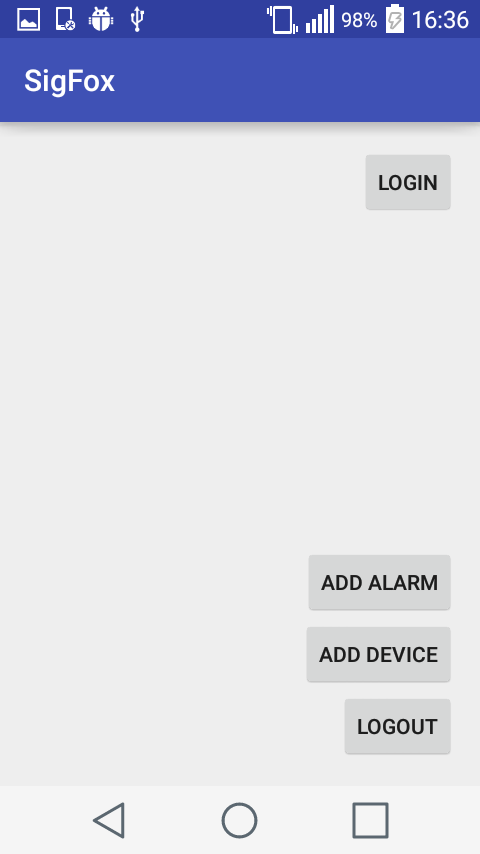
\includegraphics[width=\linewidth]{logs.png}
  \caption{Actividade \textit{Logs}}\label{fig:logs}
\endminipage\hfill
\minipage{0.29\textwidth}%
  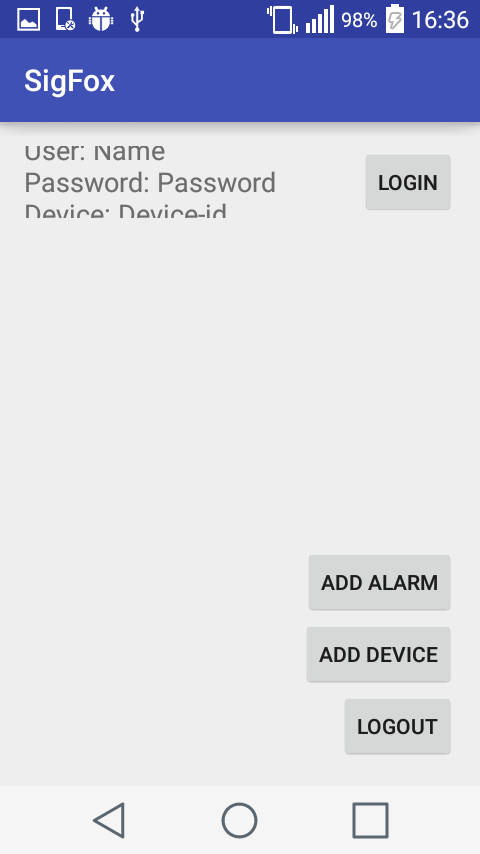
\includegraphics[width=\linewidth]{login.png}
  \caption{Actividade \textit{Logs} com \textit{login}}\label{fig:login}
\endminipage
\end{figure}

Relativamente à obtenção das leituras do sensor de arduíno a partir da \textit{Cloud Sigfox}, foi realizado um programa à parte por forma a testar apenas esta funcionalidade, tal como representado nas figuras abaixo. O programa, além de recolher os dados, realiza o \textit{parse} do \textit{JSON}.

\begin{figure}[H]
\minipage{0.40\textwidth}
  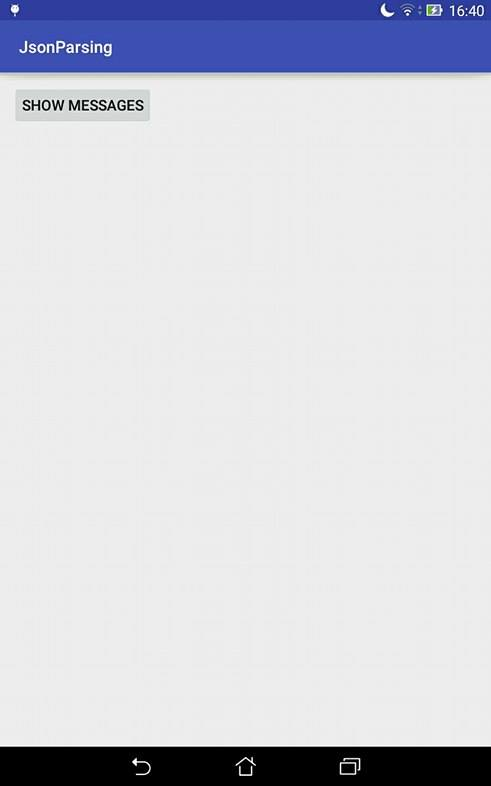
\includegraphics[width=\linewidth]{get.jpg}
  \caption{Botão para obtenção da informação da \textit{Cloud}}\label{fig:get}
\endminipage\hfill
\minipage{0.40\textwidth}
  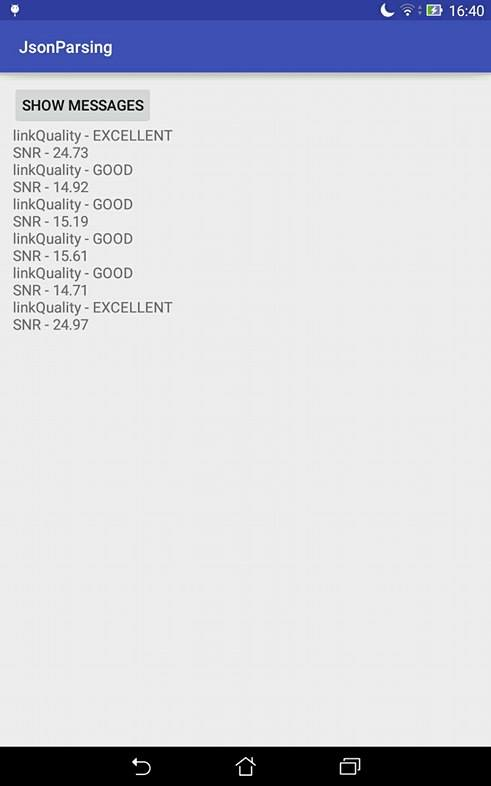
\includegraphics[width=\linewidth]{json.jpg}
  \caption{Recolha da informação com \textit{parse}}\label{fig:json}
\endminipage\hfill
\end{figure}

Será agora necessária a interligação dos dois programas e a activação das notificações, por forma a que a aplicação fique terminada.

Relativamente ao sensor, foi apenas realizado o trabalho de pesquisa, sendo iniciada a implementação quando a aplicação estiver concluída.

\section{Alterações face ao planeamento inicial}



\section{Pontos críticos}


\begin{thebibliography}{9}

\bibitem{ficheiros}
  [FILE16] \texttt{http://developer.android.com/reference/java/io/File.html}, Março 2016
  
\bibitem{thread}
  [THREAD16] \texttt{http://developer.android.com/reference/java/lang/Thread.html}, Março 2016
  
\bibitem{get}
  [HTTPURLCONNECTION16] \begin{sloppypar} \texttt{http://developer.android.com/reference/java/net/HttpURLConnection.html}, Março 2016 \end{sloppypar}
  
\bibitem{get_}
  [URLCONNECTION16] \begin{sloppypar}\texttt{http://developer.android.com/reference/java/net/URLConnection.html}, Março 2016 \end{sloppypar}
  
\bibitem{jason}
  [JSON16] \texttt{http://developer.android.com/reference/android/util/JsonReader.html}, Março 2016
  
\bibitem{notifications}
  [NOTIFICATION16] \begin{sloppypar}\texttt{http://developer.android.com/training/notify-user/build-notification.html}, Março 2016 \end{sloppypar}
  
\bibitem{Akeru}
  [AKERU16] \texttt{https://github.com/Snootlab/Akeru}, Fevereiro 2016


\end{thebibliography}

\end{document}